\documentclass[a4paper,11pt]{article}

\usepackage{amsmath}
\usepackage{amssymb}
\usepackage{booktabs}
\usepackage{caption}
\usepackage{float}
\usepackage{geometry}
\usepackage{graphicx}
\usepackage{hyperref}
\usepackage{longtable}
\usepackage{array}
\usepackage{xcolor}

\geometry{left=2.4cm,right=2.4cm,top=2.5cm,bottom=2.5cm}
\graphicspath{{../assets/}}
\hypersetup{colorlinks=true,linkcolor=black,citecolor=black,urlcolor=blue}
\captionsetup{font=small,labelfont=bf}

\title{\textbf{Experiments}\\Reproduction Report for High-Dimensional MSWD Two-Sample Testing}
\author{MSWD Bootstrapping Reproduction}
\date{\today}

\begin{document}
\maketitle

\begin{abstract}
This report summarizes the three main experiments completed in the current project, based on Hu and Lin's \textit{Biometrika} paper \textit{Two-sample distribution tests in high dimensions via max-sliced Wasserstein distance and bootstrapping}. Experiment 1 reproduces the Model A comparison behind Figure 1, using the first 50 complete Monte Carlo runs for each signal level. Experiment 2 isolates the proposed MSWD bootstrap mechanism on one generated data set per signal level. Experiment 3 reproduces the real-data LGG/GBM DNA methylation analysis. Overall, the results support the paper's main message: sparse max-sliced Wasserstein testing has strong power against high-dimensional sparse mean-shift alternatives and can provide interpretable localization through marginal genes and GO-term gene subsets.
\end{abstract}

\section{Paper Basis and Experimental Arc}

The paper studies the high-dimensional two-sample problem
\[
H_0:P=Q,\qquad H_1:P\neq Q,
\]
where \(P\) and \(Q\) are distributions on \(\mathbb{R}^p\), and \(p\) may be comparable to or larger than the sample sizes. Direct empirical Wasserstein distances suffer from the curse of dimensionality. The proposed method avoids this by projecting the data to one dimension and searching for the direction that maximizes the projected Wasserstein discrepancy.

For a projection direction \(v\), the one-dimensional Wasserstein distance is \(W_1(v^\top X,v^\top Y)\). The max-sliced Wasserstein distance is
\[
D(X,Y)=\sup_{\|v\|_2=1} W_1(v^\top X,v^\top Y).
\]
In high dimensions, the paper restricts the search to sparse directions
\[
V_{0,s}=\{v\in\mathbb{R}^p:\|v\|_2=1,\ \|v\|_0\le s\},
\]
and defines the empirical sparse max-sliced distance
\[
D_n=\sup_{v\in V_{0,s}}\sup_{f\in \mathrm{Lip}_1}
\left\{\frac{1}{n_1}\sum_{i=1}^{n_1}f(v^\top X_i)
-\frac{1}{n_2}\sum_{j=1}^{n_2}f(v^\top Y_j)\right\}.
\]
The test statistic is
\[
T_n=\left(\frac{n_1n_2}{n_1+n_2}\right)^{1/2}D_n.
\]
The null distribution is approximated by bootstrap multipliers; the null is rejected when the observed \(T_n\) exceeds the bootstrap \(1-\alpha\) quantile.

A distinctive advantage of the method is that the same bootstrap construction also yields simultaneous confidence intervals (SCIs). Therefore, after a global rejection, the method can identify significant projection directions, marginal coordinates, and coordinate subsets without running separate tests.

\section{Experiment 1: Model A Method Comparison with 50 Runs}

\subsection{Configuration}

Experiment 1 corresponds to Model A in the paper's Figure 1:
\[
X\sim N(0_p,\Sigma),\qquad Y\sim N(\mu,\Sigma),
\]
with
\[
\Sigma_{ij}=0.5^{|i-j|},\qquad \mu_j=0.8\beta j^{-3},\quad j=1,\ldots,p.
\]
The reproduction uses:

\begin{itemize}
  \item sample sizes \(n_1=n_2=250\);
  \item dimension \(p=500\);
  \item significance level \(\alpha=0.05\);
  \item signal grid \(\beta=0,0.2,0.4,0.6,0.8,1.0\);
  \item the first 50 complete Monte Carlo runs for each \(\beta\);
  \item \(B=300\) bootstrap replications for the Proposed method;
  \item L0 sparsity candidates \(\{1,5,10,20,50\}\), selected by 2-fold cross-validation;
  \item 10 random restarts for the main optimization and 1 restart inside each bootstrap computation;
  \item comparison methods MMD-G, ED$_2$, BG, and PW. MMD-L cannot be recovered from the existing logs because \texttt{main.py} did not print \texttt{lapmmd\_decision}.
\end{itemize}

The original paper used 300 independent simulation replications. Here the reported rates are based on 50 runs, as requested, and should be interpreted with Monte Carlo uncertainty.

\subsection{Results}

\begin{table}[H]
\centering
\caption{Empirical rejection rates for Model A, first 50 complete runs}
\begin{tabular}{cccccc}
\toprule
\(\beta\) & Proposed & MMD-G & ED$_2$ & BG & PW \\
\midrule
0.0 & 0.08 & 0.02 & 0.02 & 0.00 & 0.04 \\
0.2 & 0.06 & 0.02 & 0.02 & 0.02 & 0.06 \\
0.4 & 0.28 & 0.18 & 0.18 & 0.06 & 0.08 \\
0.6 & 0.84 & 0.08 & 0.08 & 0.02 & 0.08 \\
0.8 & 0.98 & 0.26 & 0.30 & 0.02 & 0.14 \\
1.0 & 1.00 & 0.58 & 0.56 & 0.08 & 0.24 \\
\bottomrule
\end{tabular}
\end{table}

\begin{figure}[H]
\centering
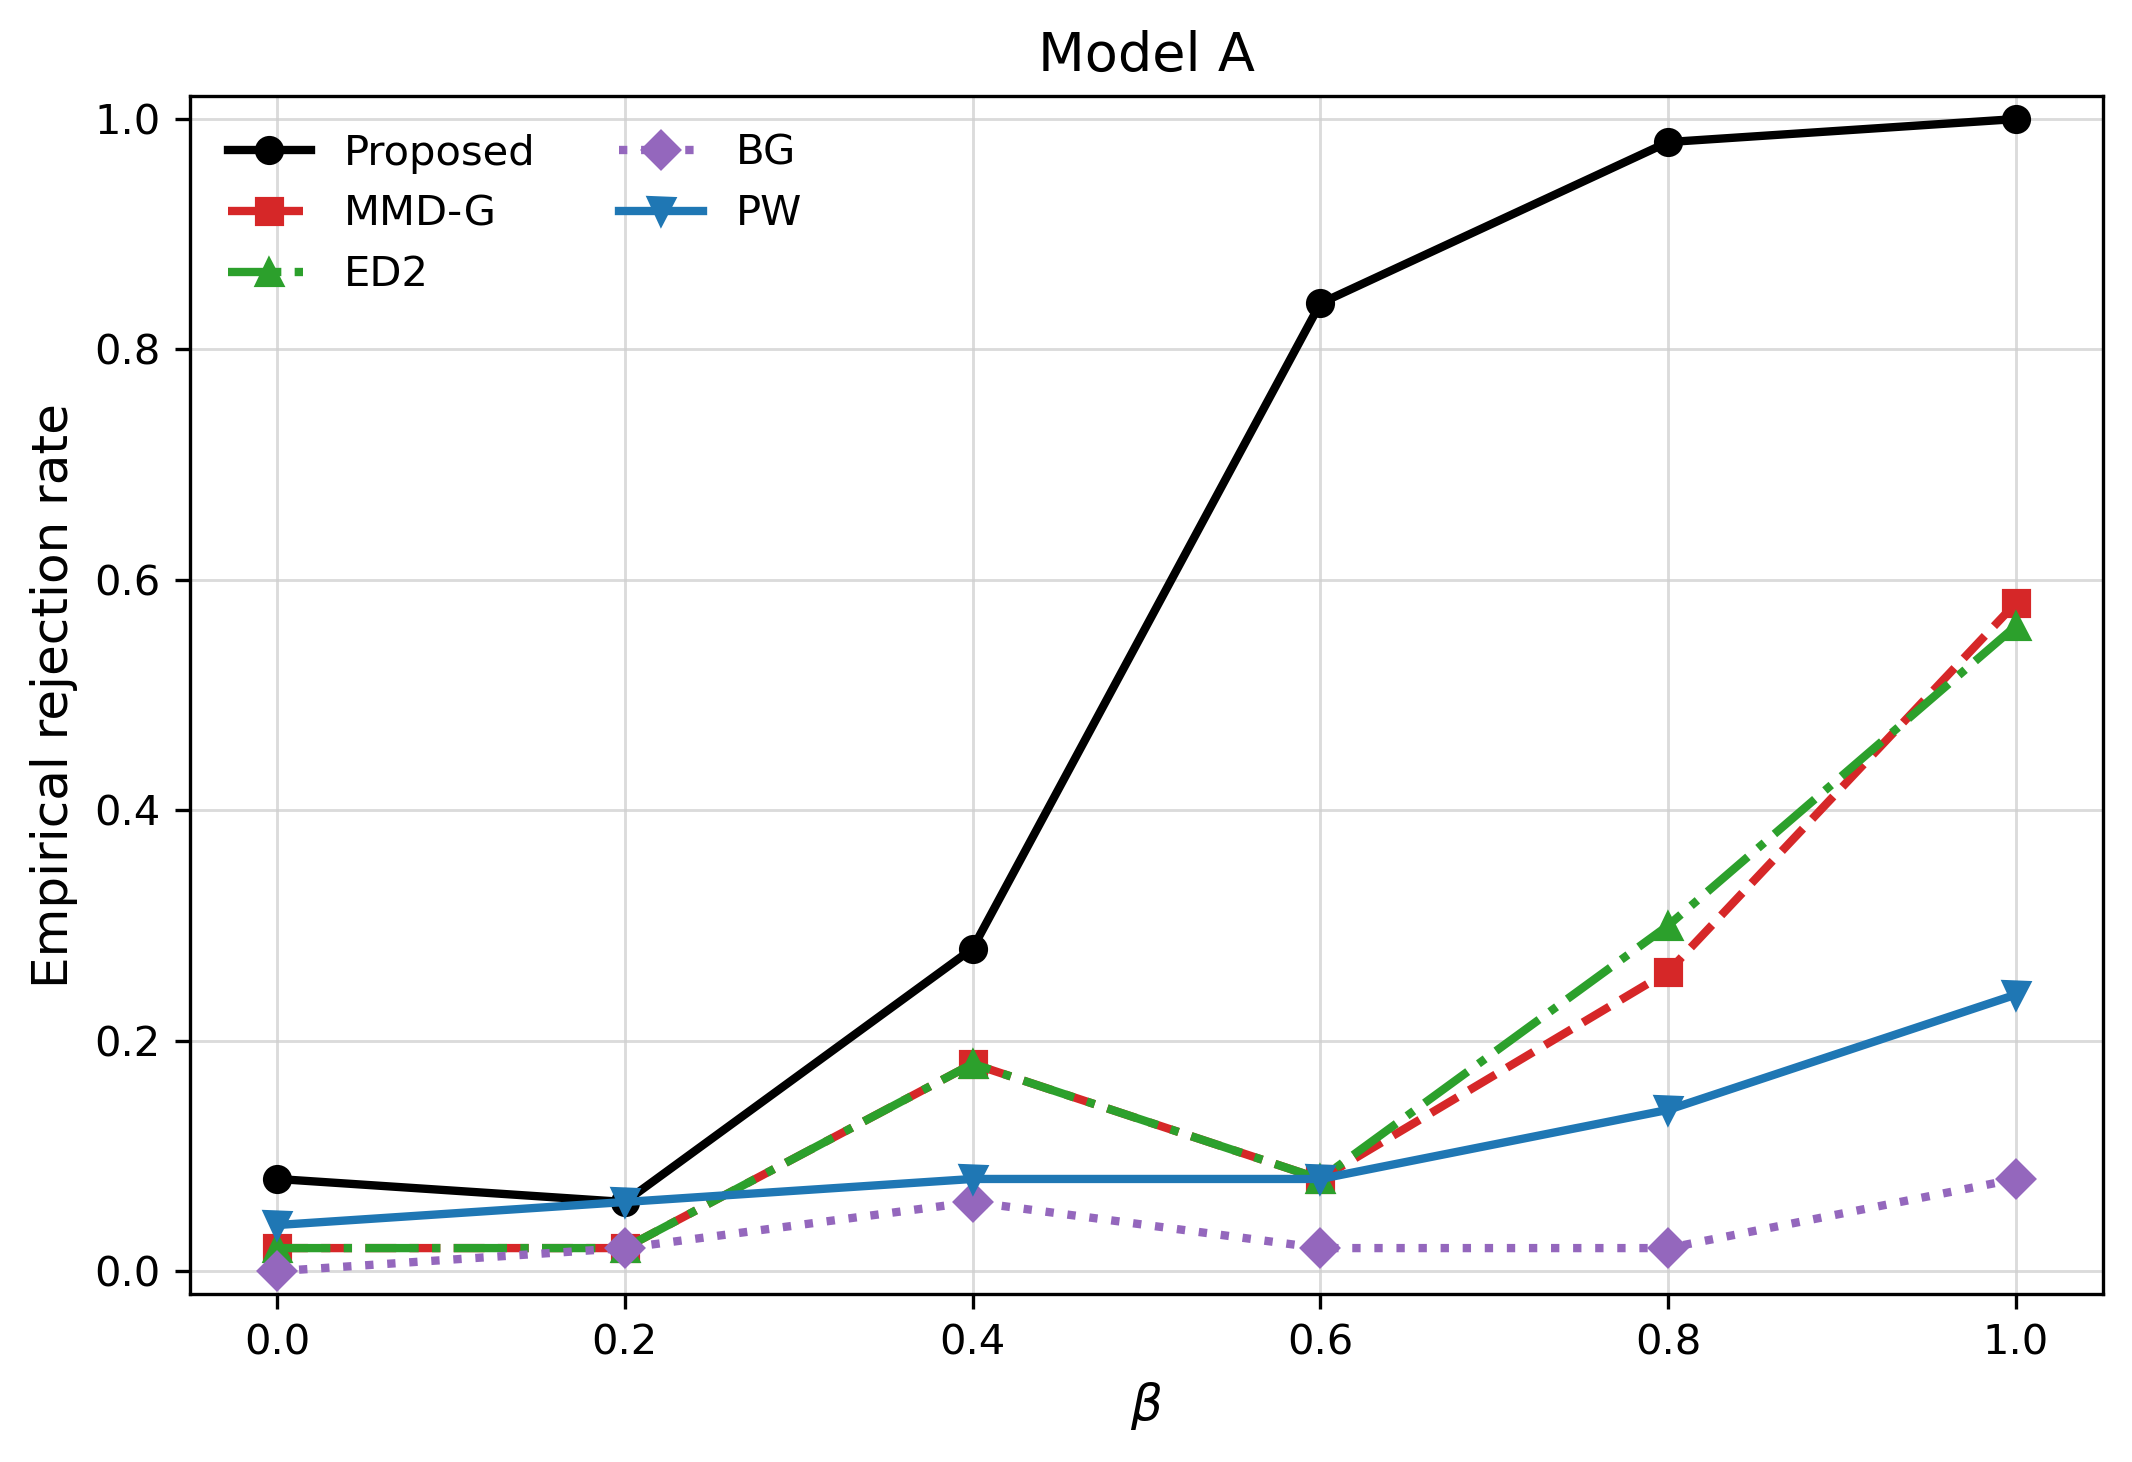
\includegraphics[width=0.86\textwidth]{fig1.png}
\caption{Empirical rejection curves for Model A, using the first 50 complete runs for each \(\beta\).}
\end{figure}

\subsection{Interpretation}

At \(\beta=0\), the two distributions are identical, so the rejection rate estimates size. The Proposed method has a size estimate of 0.08, slightly above \(\alpha=0.05\), but this is plausible under 50 Monte Carlo replications. The other methods also remain low under the null.

For \(\beta>0\), the two distributions differ through a rapidly decaying mean shift. The Proposed method's power rises sharply: 0.28 at \(\beta=0.4\), 0.84 at \(\beta=0.6\), and nearly one for \(\beta=0.8\) and \(1.0\). MMD-G and ED$_2$ improve with signal strength but remain substantially weaker; BG and PW are weaker still in this sparse decaying-mean setting.

This reproduces the main phenomenon in the paper's Figure 1: max-type sparse MSWD testing is particularly effective when the signal is concentrated in a small number of informative directions.

\section{Experiment 2: MSWD-Only Bootstrap Demonstration}

\subsection{Configuration}

Experiment 2 isolates the Proposed method. It does not estimate power. For each \(\beta\), it generates one Model A data set and then runs \(B=500\) bootstrap replications to compare the observed statistic with the bootstrap null distribution.

The configuration is
\[
n_1=n_2=250,\quad p=500,\quad \alpha=0.05,\quad B=500,
\]
\[
\beta=0,0.2,0.4,0.6,0.8,1.0,\qquad \mathrm{signal}=0.8\beta.
\]
The rejection rule is \(T_n\) greater than the 95\% bootstrap quantile.

\subsection{Results}

This report uses the final summary file \path{data/mswd_modelA_single_bootstrap_summary.csv}.

\begin{table}[H]
\centering
\caption{Observed MSWD statistic versus bootstrap threshold}
\begin{tabular}{cccccc}
\toprule
\(\beta\) & signal & observed \(T_n\) & threshold & p-value & reject \\
\midrule
0.0 & 0.00 & 3.442 & 3.885 & 0.238 & no \\
0.2 & 0.16 & 3.372 & 3.958 & 0.372 & no \\
0.4 & 0.32 & 3.256 & 3.918 & 0.484 & no \\
0.6 & 0.48 & 10.557 & 10.920 & 0.106 & no \\
0.8 & 0.64 & 7.319 & 4.025 & 0.000 & yes \\
1.0 & 0.80 & 9.479 & 3.921 & 0.000 & yes \\
\bottomrule
\end{tabular}
\end{table}

\begin{figure}[H]
\centering
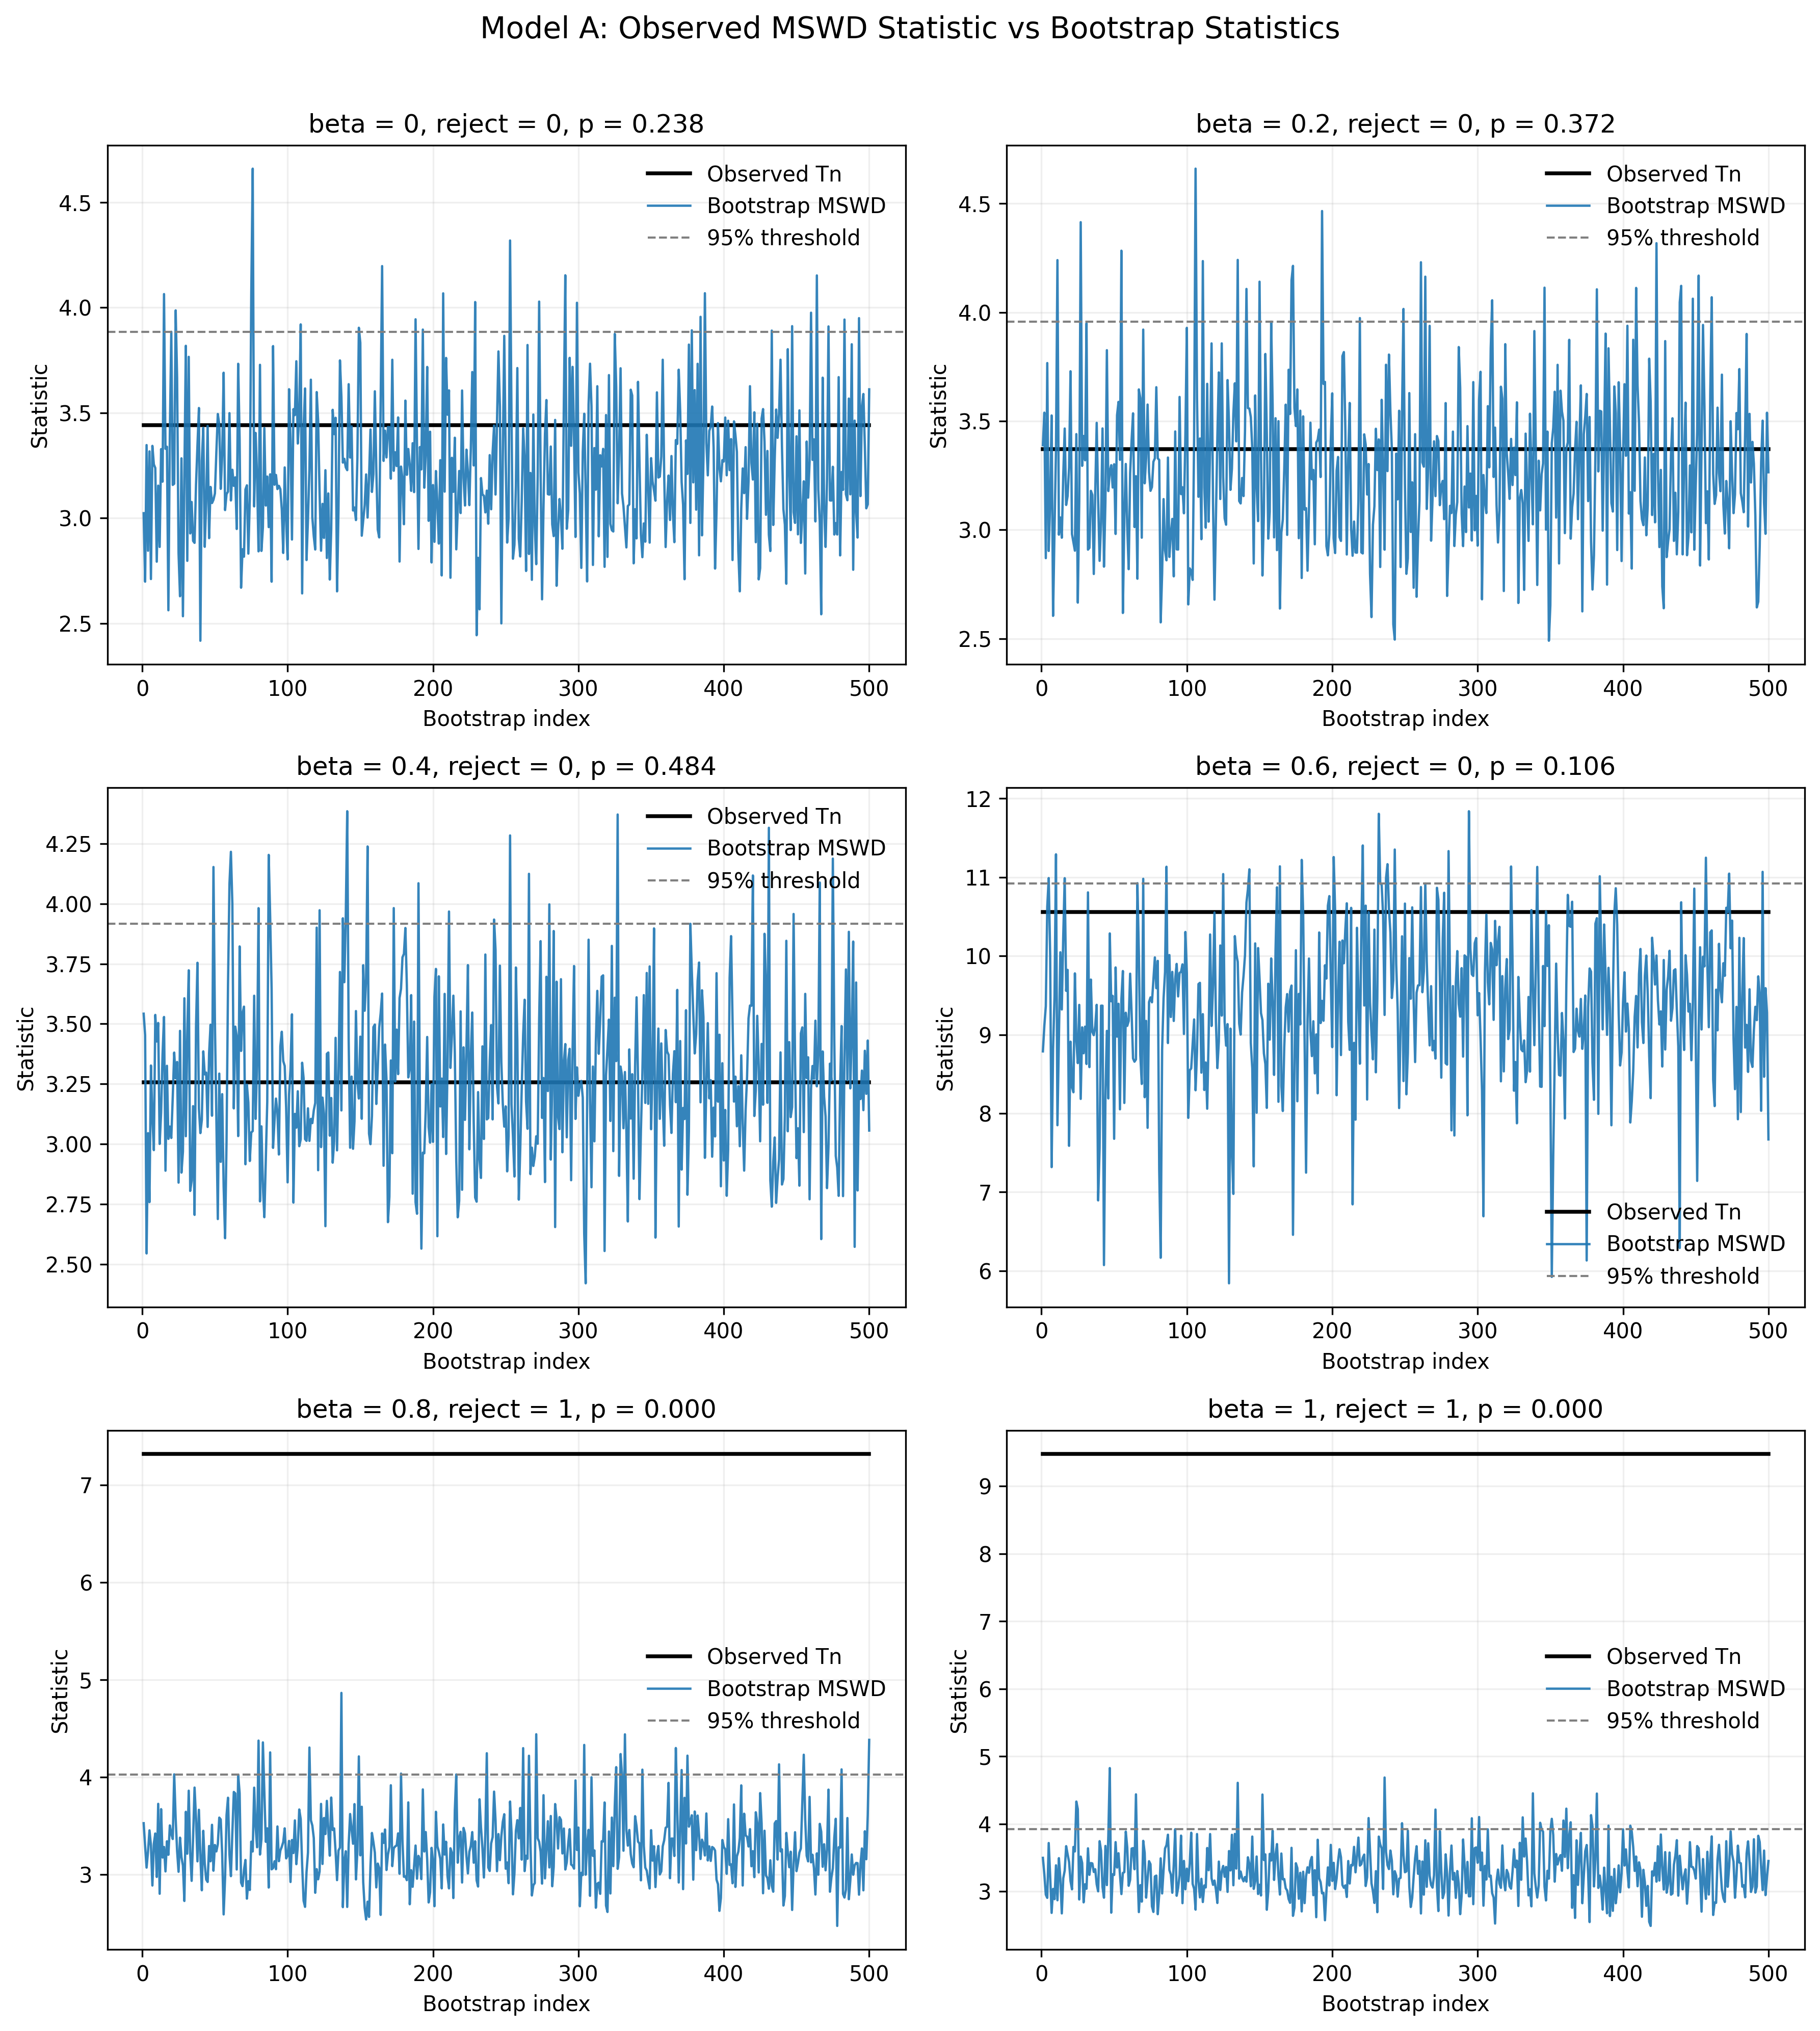
\includegraphics[width=0.92\textwidth]{fig2.png}
\caption{Observed statistic, bootstrap samples, and 95\% bootstrap threshold for each signal level.}
\end{figure}

\subsection{Interpretation}

The experiment illustrates the operational logic of the bootstrap test. For \(\beta=0,0.2,0.4\), the observed statistics are below the bootstrap thresholds. For \(\beta=0.6\), the statistic is large but remains slightly below the threshold, producing a borderline non-rejection. For \(\beta=0.8\) and \(1.0\), the observed statistics exceed the thresholds clearly. Since \(B=500\), p-values reported as zero should be interpreted as \(p<0.002\).

This single-data-set experiment is consistent with Experiment 1. Experiment 1 estimates rejection probability across 50 independent runs; Experiment 2 displays one draw per \(\beta\). A non-rejection at \(\beta=0.6\) in one generated data set is compatible with an empirical power of 0.84 across repeated runs.

\section{Experiment 3: LGG/GBM DNA Methylation Analysis}

\subsection{Configuration}

Experiment 3 reproduces the paper's real-data analysis. The data come from TCGA lower-grade glioma and glioblastoma multiforme studies, restricted to candidate prognostic genes related to glioma in the Human Pathology Atlas. After preprocessing:
\[
n_1=511\quad(\mathrm{LGG}),\qquad n_2=150\quad(\mathrm{GBM}),\qquad p=207.
\]
The hypotheses are
\[
H_0:\text{LGG and GBM have the same 207-dimensional methylation distribution},
\]
\[
H_1:\text{the two methylation distributions differ}.
\]
The reproduction uses \(\alpha=0.05\), \(B=500\), and a cross-validated L0 sparsity parameter of approximately 50.

\subsection{Global Test}

\begin{table}[H]
\centering
\caption{Global two-sample test for LGG versus GBM}
\begin{tabular}{lc}
\toprule
Metric & Value \\
\midrule
LGG sample size & 511 \\
GBM sample size & 150 \\
Gene dimension & 207 \\
Bootstrap replications & 500 \\
Selected L0 sparsity parameter & 50.0000 \\
MSWD distance & 3.9860 \\
Test statistic & 42.9236 \\
Bootstrap critical value & 1.8479 \\
Empirical p-value & 0.0, i.e. \(p<0.002\) \\
Reject \(H_0\) & yes \\
\bottomrule
\end{tabular}
\end{table}

The observed statistic is far above the bootstrap threshold, so the LGG and GBM DNA methylation distributions differ significantly. This agrees with the paper's reported \(p<10^{-3}\).

\subsection{Marginal Genes and GO-Term Gene Sets}

Using the SCI mechanism, the reproduction identifies
\[
138/207
\]
prognostic genes with significant marginal methylation differences. The paper reports 139 genes; the one-gene discrepancy is plausible given bootstrap randomness, non-convex optimization, and software/runtime differences.

\begin{table}[H]
\centering
\caption{GO biological process gene-set analysis}
\begin{tabular}{lccc}
\toprule
GO term & Genes & Statistic & Significant \\
\midrule
mitotic\_cell\_cycle & 5 & 9.467 & yes \\
mitotic\_cell\_cycle\_process & 4 & 9.465 & yes \\
cell\_cycle\_process & 7 & 10.196 & yes \\
cell\_cycle & 11 & 15.454 & yes \\
DNA\_metabolic\_process & 6 & 8.730 & yes \\
cell\_division & 5 & 11.126 & yes \\
mitotic\_nuclear\_division & 3 & 4.131 & yes \\
\bottomrule
\end{tabular}
\end{table}

All seven GO biological process subsets are significant, localizing the LGG/GBM difference to cell-cycle, DNA-metabolic, cell-division, and mitotic processes.

\begin{figure}[H]
\centering
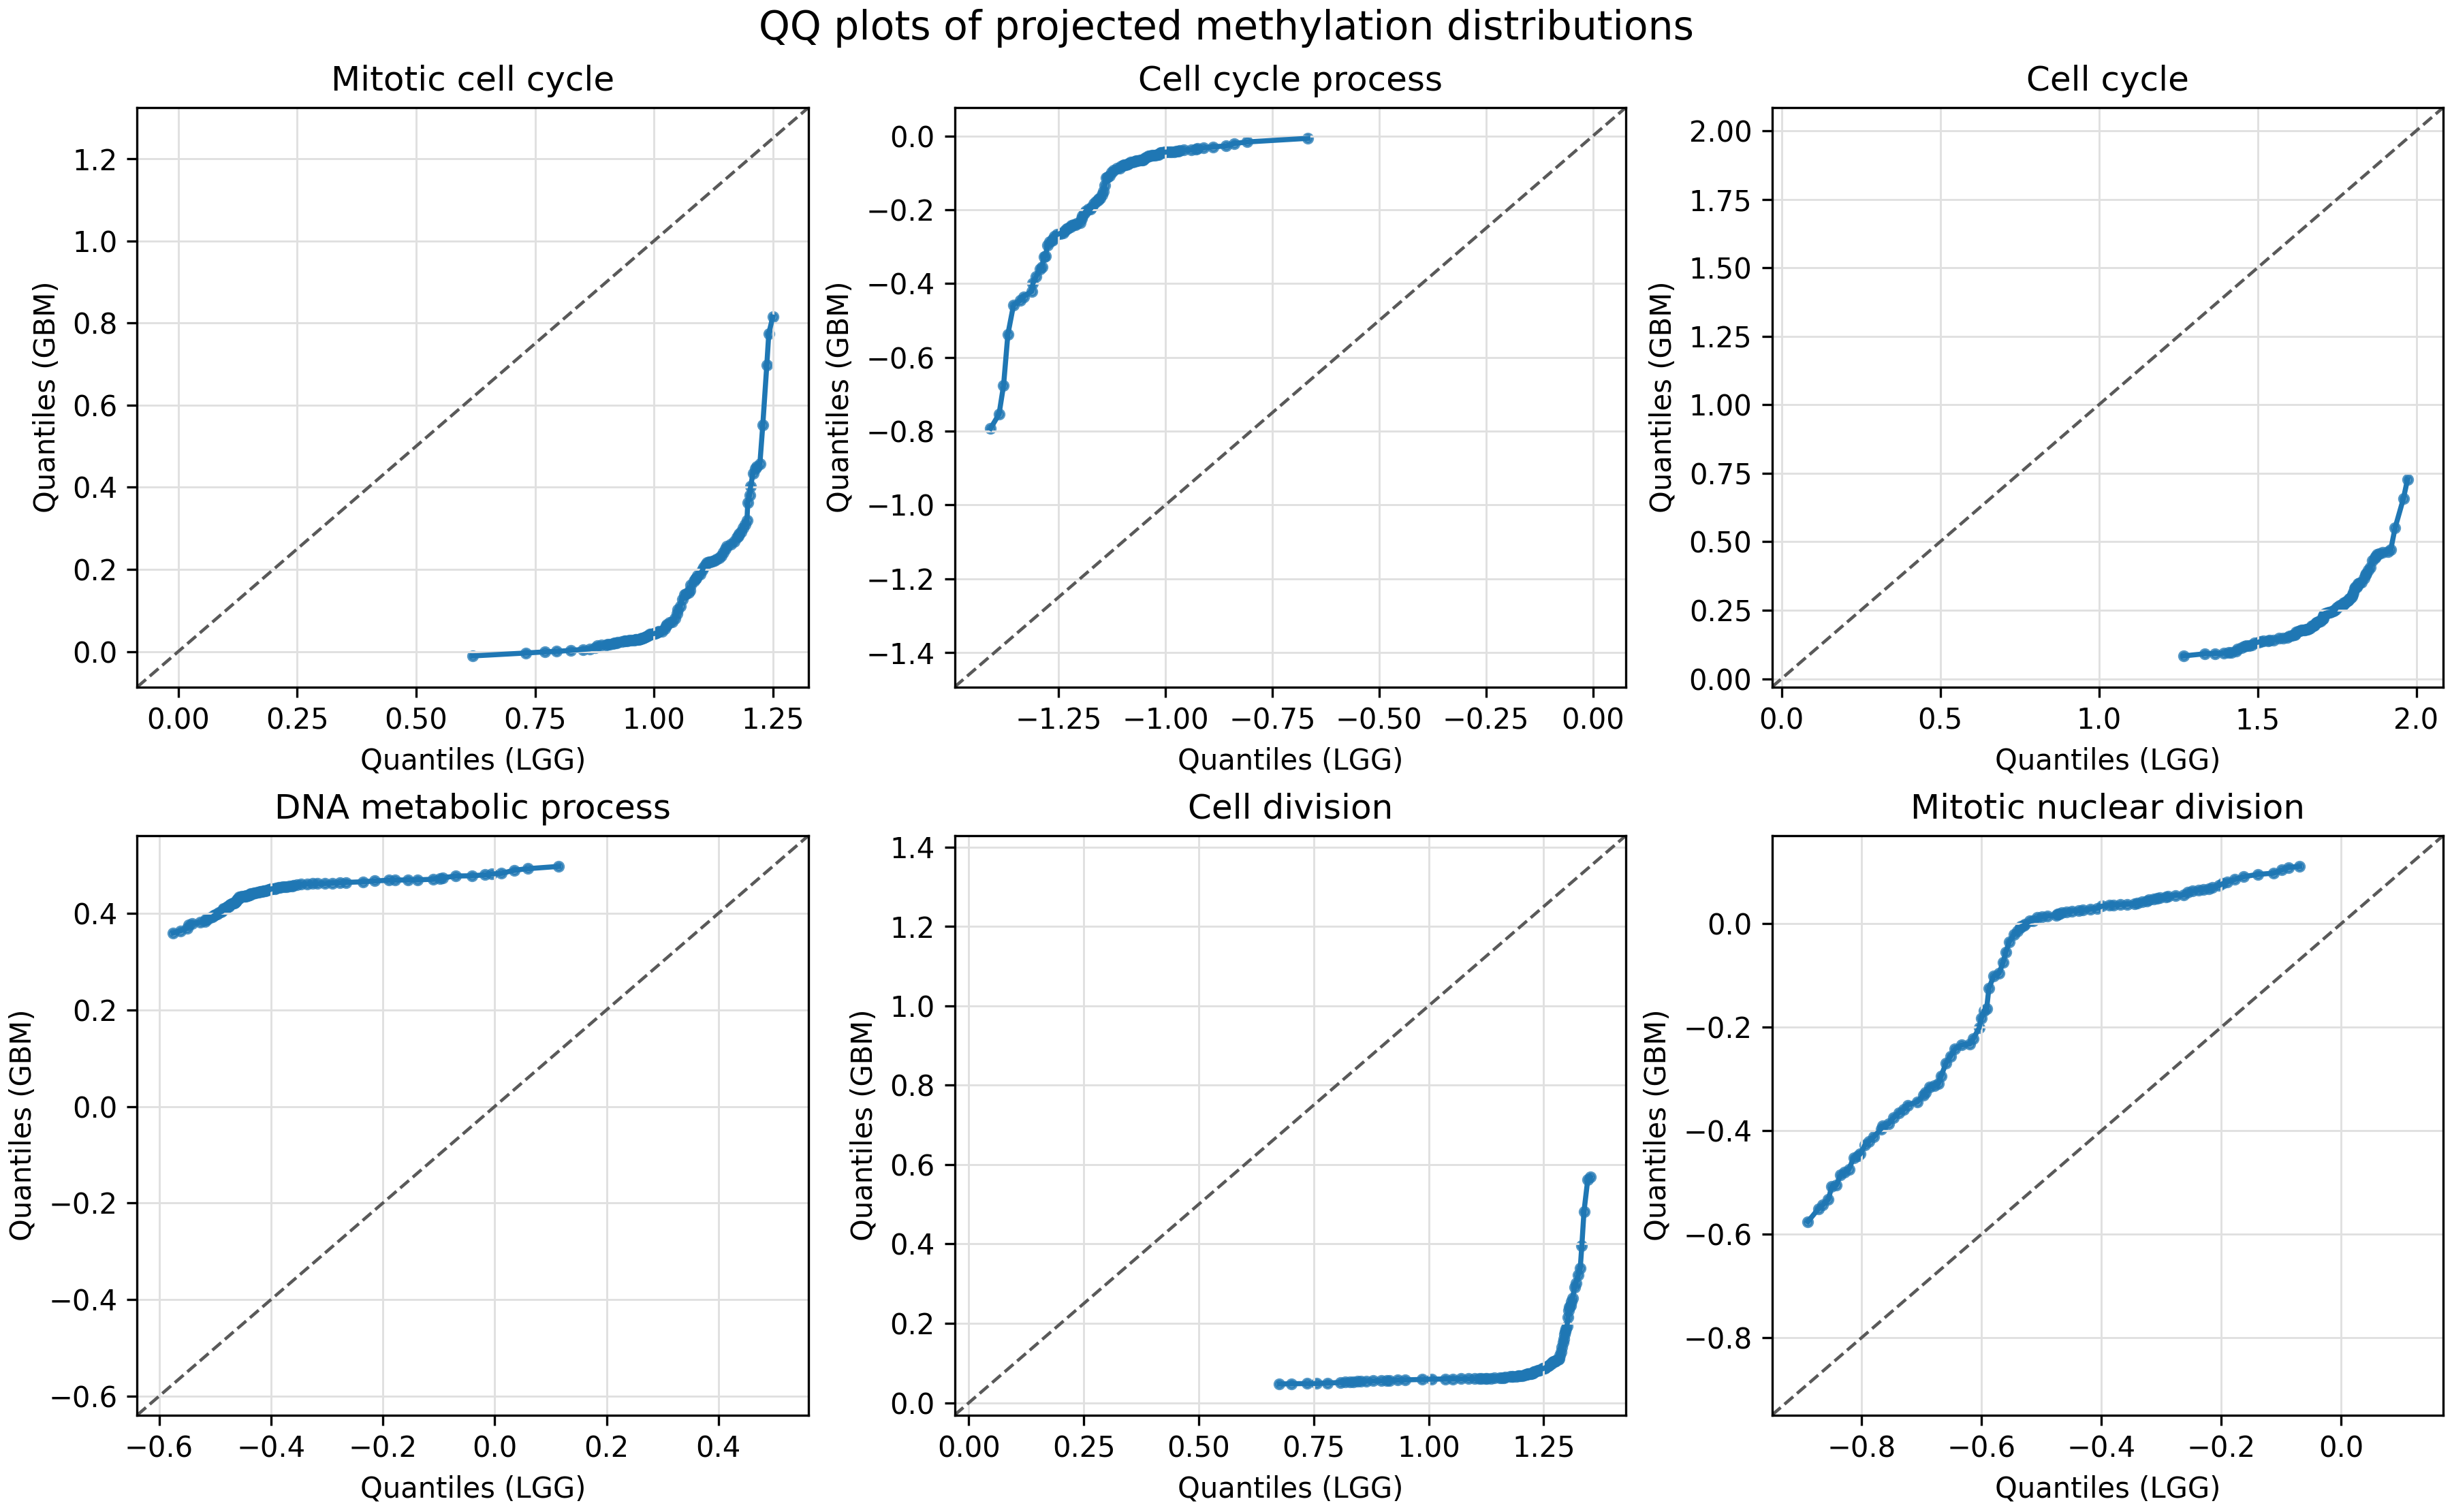
\includegraphics[width=0.88\textwidth]{fig3.png}
\caption{QQ plots for LGG and GBM after projecting each GO-term gene subset onto its maximal MSWD direction. Departure from \(y=x\) indicates distributional difference.}
\end{figure}

The QQ plots support the gene-set table: every panel visibly departs from the identity line. The exact visual shape may differ from the paper because \(v\) and \(-v\) are equivalent maximal directions and because the optimization is non-convex. These differences do not change the test statistic or significance interpretation.

\section{Integrated Understanding}

The three experiments form a coherent evidence chain. Experiment 1 asks whether the method has a power advantage in the core simulation setting; the answer is yes, especially for sparse decaying mean shifts. Experiment 2 shows how the bootstrap decision is made for the Proposed statistic: compare the observed \(T_n\) to the bootstrap null quantile. Experiment 3 shows that the method is useful beyond simulation, detecting a strong global methylation difference between LGG and GBM and localizing the difference to interpretable marginal genes and biological processes.

Statistically, the advantage of MSWD comes from two design choices. First, the max-sliced construction searches for the most informative projection rather than averaging weak signals over all directions. Second, the bootstrap and SCI framework connects global testing with post-rejection localization, giving a unified inferential procedure for high-dimensional biological data.

\section{Reproduction Files}

The figures and data used in this report have been copied into the report directory:

\begin{itemize}
  \item Experiment 1: \path{data/modelA_first50_summary.csv}, \path{assets/fig1.png};
  \item Experiment 2: \path{data/mswd_modelA_single_bootstrap_summary.csv}, \path{assets/fig2.png};
  \item Experiment 3: \path{data/GBM_global_test_summary.txt}, \path{data/GBM_gene_set_summary.txt}, \path{data/GBM_grade_marginal_summary.txt}, \path{assets/fig3.png};
  \item Source paper: \path{data/source_paper.pdf}.
\end{itemize}

\begin{thebibliography}{9}
\bibitem{HuLin2025}
Hu, X. and Lin, Z. (2025).
\textit{Two-sample distribution tests in high dimensions via max-sliced Wasserstein distance and bootstrapping}.
Biometrika, 112(2), asaf001.
\end{thebibliography}

\end{document}
